%%%
%
% Purpose of this document
%
% This note gives an outline for the structure of a plan for a Master's project for the Master in
% Software Engineering. Each student should produce a plan according to the template given below,
% discuss it with the supervisors and the host (if applicable) and get it approved via DataNose by
% the academic supervisor and thesis coordinator (Martin Bor, m.c.bor@uva.nl).
%
%%%
\documentclass[conference,a4paper]{IEEEtran}

\usepackage[british]{babel}
\usepackage{pgfplots}
\usepackage{cite}
\usepackage{dblfloatfix}
\usepackage{url}
\urlstyle{same}
\usepackage{booktabs}
\usepackage{amssymb}
\usepackage{graphicx}
\pgfplotsset{compat=1.18}


\title{Streaming Communication for Scalable Data Exchange in DYNAMOS}
\author{%
\IEEEauthorblockN{Ruben Stoop}
\IEEEauthorblockA{Complex Cyber-Infrastructure (CCI)\\
University of Amsterdam\\
Amsterdam, the Netherlands}
}

\begin{document}

\maketitle

\begin{abstract}
This thesis investigates how streaming communication can be introduced into DYNAMOS, a policy-driven middleware for data exchange based on dynamically composed microservices. The current system relies on unary gRPC request-response interactions, which become increasingly inefficient for large or continuous transfers. To ground the broader architectural and comparative study, the thesis first reviews candidate streaming mechanisms and evaluates them in a controlled \emph{Producer} $\rightarrow$ \emph{Transformer} $\rightarrow$ \emph{Sink} pipeline. The current empirical results now compare client-streaming gRPC, unary gRPC, and RabbitMQ Streams across clean bulk transfer, paced continuous delivery, slow-consumer overload, forced-restart recovery, and resource cost. In the completed single-repeat benchmark suite, client-streaming provides the highest sustained throughput, unary keeps the lowest per-message latency in the direct RPC path, and RabbitMQ Streams preserves correctness in the clean matrices but operates at much lower throughput and much higher end-to-end latency. These findings define the current trade-off space for brokered versus direct streaming in DYNAMOS and motivate the remaining cross-broker comparison and system-integration work.
\end{abstract}

\begin{IEEEkeywords}
streaming communication, microservices, gRPC, event streaming, policy-driven middleware, DYNAMOS
\end{IEEEkeywords}

\section{Introduction}

Many contemporary distributed systems operate in environments where data and computational resources are owned by different organizations. In such settings, data exchange must adhere to legal agreements, privacy regulations, and organizational policies. These constraints are common in domains such as healthcare, scientific research, and public-sector infrastructures, where unrestricted data exchange is not acceptable.

DYNAMOS (Dynamically Adaptive Microservice-based Operating System) is a data exchange middleware developed by the Complex Cyber-Infrastructure (CCI) group at the University of Amsterdam. The system implements a set of recurring data sharing archetypes that describe how data and computation are distributed among participants under policy constraints. DYNAMOS realizes these archetypes by dynamically composing chains of microservices that execute data sharing requests in compliance with formally evaluated policies. The middleware is designed to be adaptive, allowing architectural and execution decisions to change at runtime in response to policy requirements.

The current implementation of DYNAMOS uses gRPC for inter-service communication and relies exclusively on atomic request--response interactions. This communication model is suitable for small or bounded data transfers but becomes limiting when applied to large-scale or continuous data exchange. In practice, data in distributed systems is often produced and consumed incrementally, for example in sensor data streams, distributed analytics pipelines, or staged processing of large research datasets.

When request--response communication is used in such scenarios, systems must either buffer large volumes of data before transmission or split transfers into multiple independent requests. Buffering increases memory usage and can lead to idle time between producers and consumers. Repeated request--response interactions introduce additional coordination overhead. Both effects negatively impact scalability and resource utilization as data volumes and the number of participating services increase.

Streaming-based communication has been proposed as a solution to these limitations. Streaming allows data to be transferred and processed incrementally, enabling overlap between computation and communication and reducing peak memory usage. gRPC supports several streaming interaction patterns, including client-side, server-side, and bidirectional streaming.

Integrating streaming communication into DYNAMOS is not straightforward. Streaming relies on long-lived connections and continuous data flows, which must be reconciled with DYNAMOS' policy-driven execution model, dynamic microservice composition, orchestration decisions, and fault handling mechanisms. Without careful design, the introduction of streaming may interfere with policy enforcement or reduce the ability to evaluate and reason about system behavior.

The goal of this thesis is to investigate how streaming communication can be incorporated into DYNAMOS in a way that improves scalability and performance while preserving policy compliance and adaptive behavior. This involves analyzing existing streaming communication mechanisms, designing architectural extensions to the middleware, implementing streaming support, and evaluating the resulting system under realistic workloads.

The main research question addressed in this thesis is how streaming communication can be integrated into a dynamically adaptive, policy-driven microservice-based data exchange middleware such as DYNAMOS while preserving compliance guarantees and improving scalability and performance. To answer this overarching question, the thesis is structured around three sub-questions: which streaming communication technologies, frameworks, and interaction patterns are suitable for large-scale and continuous data exchange in microservice-based systems such as DYNAMOS; how streaming communication can be integrated into a microservice-based architecture while preserving dynamic service composition, policy-driven orchestration, and isolation guarantees; and what impact streaming communication has on scalability, performance, and robustness compared to a traditional request--response approach under realistic workloads in a microservice-based architecture.

The present document concentrates on the first empirical step in that broader programme. It narrows the design space through a literature-guided comparison, defines a reproducible benchmark for DYNAMOS-relevant streaming workloads, and reports the current three-transport benchmark results for client-streaming gRPC, unary gRPC, and RabbitMQ Streams. Later thesis stages build on this comparison by extending the broker evaluation set and by evaluating architectural fit inside DYNAMOS itself.

\section{Related Work}

This section reviews existing literature related to streaming communication in microservice-based systems, with a particular focus on topics that are central to this thesis: streaming communication technologies and interaction models, architectural integration in adaptive microservice middleware, policy enforcement under continuous data exchange, resilience mechanisms for streaming workflows, and validation practices with respect to scalability and performance.

\subsection{Streaming communication technologies and interaction models}

DYNAMOS is implemented as a dynamically composed microservice system deployed on Kubernetes, using gRPC for inter-service communication and RabbitMQ for asynchronous messaging \cite{stutterheim2023thesis,stutterheim2023icsa}. This constrains the design space for introducing streaming functionality to a limited set of technologies that are compatible with containerized microservices and cloud-native deployment models. The primary question addressed in this body of work is which streaming communication mechanisms are suitable for large-scale or continuous data exchange, and under which conditions direct streaming RPC should be preferred over broker-based approaches.

gRPC provides native support for streaming through client-streaming, server-streaming, and bidirectional streaming RPCs. These interaction patterns differ in message flow control, lifetime of connections, buffering behaviour, and error propagation semantics. In the context of DYNAMOS, the choice of streaming pattern is not merely an API concern but has architectural consequences, as it affects memory usage, cancellation behaviour, and the ability to overlap communication and computation. The original DYNAMOS thesis identifies client-streaming as a promising mechanism for transferring large datasets incrementally, reducing peak memory pressure at the cost of increased handling complexity \cite{stutterheim2023thesis}.

However, the use of long-lived streaming connections introduces operational challenges that are largely absent in unary request--response interactions. Starck and Ghofrani show that gRPC streaming complicates load balancing in Kubernetes environments, as persistent connections can cause traffic to become unevenly distributed across replicas \cite{starck2023streaminglb}. This observation is particularly relevant for systems such as DYNAMOS that rely on horizontal scaling and ephemeral execution units. Complementary benchmarking work demonstrates that the performance characteristics of streaming gRPC are sensitive to runtime configuration and virtualization overhead, with measurable effects on latency and resource utilisation in containerized environments \cite{sodankoor2026grpcbench}.

An alternative to direct service-to-service streaming is to externalise the data plane to a messaging or event streaming platform. Broker-based communication decouples producers and consumers in time, delegates buffering and persistence to the broker, and can simplify fan-out scenarios. Comparative benchmarks of Kafka, RabbitMQ, NATS, and ActiveMQ Artemis show that different brokers dominate under different workload characteristics, reinforcing that broker choice is highly workload dependent \cite{ibrahim2026brokers}. A cloud-native literature review comparing Kafka, Pulsar, and RabbitMQ further highlights trade-offs between throughput, reliability, operational complexity, and Kubernetes integration \cite{nuikka2021cloudnative}. While these studies are not conducted in the context of policy-driven middleware, they provide structured criteria that are directly applicable when evaluating broker-based alternatives for DYNAMOS.

Several studies also emphasize that streaming design is influenced not only by technology choice but by the underlying communication model. DataXc contrasts push-based streaming approaches with pull-based designs and reports improved latency stability and throughput under consumer-controlled flow \cite{coviello2022dataxc}. Although the application domain differs, the distinction between producer-driven and consumer-driven streaming is directly relevant to backpressure management and resource utilisation in DYNAMOS-compatible workflows.

Overall, existing literature provides a broad comparison of streaming technologies and interaction patterns, but these comparisons are typically conducted in generic microservice or stream-processing settings. There is limited work that evaluates these mechanisms under the specific constraints of dynamically composed, policy-driven middleware with ephemeral execution units, leaving open questions regarding their suitability in such environments.

\subsection{Architectural integration of streaming in adaptive microservice middleware}

Beyond the selection of a streaming mechanism, integrating streaming communication into an adaptive microservice architecture raises architectural questions related to modularity, orchestration, and lifecycle management. DYNAMOS is explicitly designed around dynamic microservice composition, where execution chains are generated and deployed per request based on policy evaluation and system state \cite{stutterheim2023thesis,stutterheim2023icsa}. These chains are short-lived by design, which improves isolation and compliance guarantees but complicates the management of long-lived communication channels.

Communication in DYNAMOS is abstracted through a sidecar-based architecture, decoupling communication concerns from core microservice logic. The sidecar pattern is widely used in cloud-native systems to address cross-cutting concerns such as observability, security, and traffic management. Figueira and Coutinho demonstrate how sidecars can be integrated into self-adaptive microservice architectures on Kubernetes, enabling runtime adaptation without violating service modularity \cite{figueira2024selfadaptive}. While their work does not explicitly address streaming data transfer, it illustrates how communication behaviour can be adapted dynamically at runtime.

Several middleware frameworks operationalise sidecars as first-class runtime components. Dapr provides a protocol-agnostic communication abstraction that supports service invocation, pub/sub, and state management through a sidecar runtime \cite{figueira2024selfadaptive}. Dapr demonstrates that heterogeneous communication paradigms, including streaming and messaging, can be unified behind a stable interface. However, Dapr assumes relatively static service topologies and does not address dynamic chain composition driven by policy evaluation, limiting its applicability as a direct solution for DYNAMOS.

Existing architectural work therefore supports the feasibility of integrating streaming into sidecar-based microservice systems but does not address the combination of long-lived streaming connections with ephemeral, dynamically composed execution chains. This limitation is particularly relevant in systems that combine adaptivity with strict policy enforcement requirements.

\subsection{Policy enforcement and compliance under continuous data exchange}

Policy enforcement is a defining characteristic of DYNAMOS, where access rights, execution locations, and data-flow constraints are evaluated prior to execution and enforced through dynamically composed microservice chains \cite{stutterheim2023thesis,stutterheim2023icsa}. In the current architecture, policy enforcement is implicitly scoped to bounded request--response interactions. Introducing streaming communication challenges this assumption, as data transfer may span longer periods during which policies, system state, or execution context may change.

Neumaier et al. propose a policy-aware architecture for decentralized dataset exchange that emphasizes continuous monitoring and runtime validation against machine-readable policies \cite{neumaier2021policyaware}. While their work does not explicitly target streaming RPC, it introduces an important distinction between one-time policy clearance and ongoing compliance monitoring, which becomes critical when data is exchanged incrementally over long-lived connections.

At the communication layer, several studies propose enforcing security and access control through proxies or sidecars. Thiyagarajan et al. present a proxy-based approach for securing gRPC communication using mTLS, JWT authentication, and RBAC \cite{thiyagarajan2025grpcsecurity}. Although the focus is on security rather than data usage policy, the architectural approach is relevant, as it suggests that enforcement can be applied at communication boundaries and potentially at message granularity.

Despite these contributions, there is limited guidance on how policy enforcement should interact with long-lived streaming connections in systems that dynamically compose execution chains. In particular, existing work does not address how policy violations should be detected or handled mid-stream, or how streams should be terminated or adapted when compliance conditions change. These limitations highlight open challenges when introducing streaming into policy-driven middleware such as DYNAMOS.

\subsection{Resilience, backpressure, and fault handling in streaming workflows}

Streaming-based communication introduces operational challenges that are less pronounced in request--response systems. Long-lived data flows must tolerate partial failures, adapt to fluctuating load, and prevent uncontrolled resource growth through effective backpressure mechanisms. These challenges are compounded in DYNAMOS by dynamic microservice composition and ephemeral execution units.

Reactive microservice architectures emphasize asynchronous communication, non-blocking execution, and fault isolation as mechanisms for improving resilience under variable load \cite{rasheedh2021reactive}. Although this work does not focus on streaming RPC, its principles are directly applicable to streaming workflows, where failures and backpressure must be managed continuously rather than per request.

Studies on high-volume data processing in microservices highlight the importance of explicit flow control and decoupling between producers and consumers. Guntupalli and Vamshi show that event-driven architectures combined with messaging systems can mitigate bottlenecks and stabilize performance under sustained data rates \cite{guntupalli2023highvolume}. While these systems typically rely on brokers rather than direct streaming RPC, they reinforce the need for explicit backpressure mechanisms in streaming data paths.

From a systems perspective, Gan and Delimitrou demonstrate that communication overhead and tail latency dominate the performance of large-scale microservice deployments \cite{gan2018architectural}. Their findings underline that resilience and scalability issues often emerge from inter-service communication rather than computation, an effect that is amplified in streaming scenarios.

Existing literature provides well-established principles for resilience and fault tolerance in microservice systems, but these are typically studied either in request-oriented architectures or broker-based streaming platforms. There is limited work examining how these mechanisms interact with direct streaming RPC in dynamically composed microservice chains, leaving questions about how failures and backpressure should be handled in dynamically composed microservice systems.

\subsection{Validation practices, scalability, and performance evaluation}

Empirical evaluation of streaming communication often focuses on comparing streaming and non-streaming interaction styles in terms of throughput, latency, and resource usage. Several benchmarking studies show that streaming RPCs outperform unary calls for large payloads and continuous data flows by enabling incremental processing and reducing buffering overhead \cite{sodankoor2026grpcbench}. Similar conclusions are drawn in broader comparisons between REST and gRPC, where binary protocols combined with streaming semantics demonstrate superior performance under load \cite{restgrpccomparison,lahtevenoja2021communication}.

Scalability in containerized streaming systems has been studied through systematic mapping and empirical evaluations. A mapping study on performance analysis techniques for streaming workloads in containerized microservices identifies network contention, scheduling overhead, and coordination costs as primary scalability bottlenecks \cite{systematicstreaming}. Empirical studies of streaming pipelines deployed on Kubernetes further show that streaming approaches scale more gracefully than request-response models when concurrency increases, provided that backpressure and flow control are properly configured \cite{starck2023streaminglb}.

However, most existing evaluations assume static microservice topologies and fixed execution paths. Prior performance studies rarely consider adaptive middleware that dynamically constructs execution chains based on policy evaluation. As a result, there is limited empirical insight into how streaming communication scales when embedded within dynamically adaptive, policy-driven systems such as DYNAMOS. This lack of combined evaluation of streaming, scalability, and adaptivity motivates the experimental focus of this thesis.

\section{Candidate Mechanisms and Benchmark Design}

This section addresses \emph{RQ1}: which streaming communication technologies, frameworks, and interaction patterns are suitable for large-scale and continuous data exchange in microservice-based systems such as DYNAMOS? It combines a literature-backed comparison of candidate mechanisms with a controlled benchmark design that establishes a gRPC reference baseline before broker-based alternatives are added.

\subsection{gRPC streaming}

According to the official gRPC documentation, gRPC is based on service definitions in Protocol Buffers and supports four RPC styles: unary, server-streaming, client-streaming, and bidirectional streaming. For streaming calls, message ordering is preserved within each individual RPC, while deadlines, cancellation, metadata, and both synchronous and asynchronous APIs are supported by the runtime \cite{grpc2024coreconcepts}. These properties make gRPC streaming the most direct extension of the current DYNAMOS communication model.

For microservice chains with predominantly point-to-point data transfer, client-streaming is the most natural first candidate because it lets a sender incrementally push chunks or records to a single downstream consumer. Bidirectional streaming becomes relevant when the receiver should provide progress feedback, pacing information, or explicit acknowledgements during transfer. The main advantages of gRPC streaming are low protocol overhead, direct reuse of protobuf contracts, and the absence of an additional broker layer. The disadvantages are that sender and receiver remain temporally coupled, durable replay is not provided by default, and backlog handling or crash recovery must be implemented at application level. Even so, prior work on asynchronous gRPC streaming demonstrates that carefully designed protocols can support efficient and even exactly-once style delivery patterns, which makes gRPC a strong experimental baseline rather than merely the status-quo option \cite{roohitavaf2019logplayer,restgrpccomparison,sodankoor2026grpcbench}.

\subsection{Apache Kafka}

Apache Kafka is officially described as an open-source distributed event-streaming platform for high-performance pipelines, streaming analytics, data integration, and mission-critical applications. Its published core capabilities emphasise high throughput, durable storage, high availability, built-in stream processing, and large-scale horizontal scalability \cite{kafka2026official}. In architectural terms, Kafka exposes an append-only log abstraction in which messages are written to topics and partitions, allowing replay and independent consumption by multiple downstream readers \cite{dobbelaere2017kafkarabbitmq}.

Kafka is therefore the strongest candidate when temporal decoupling, replayability, or large consumer backlogs matter more than direct point-to-point simplicity. Its advantages are durable retention, repeated reads by independent consumers, and a mature ecosystem for analytics and downstream integration. The disadvantages are the extra operational footprint of a broker cluster, partition-local rather than global ordering, and a non-trivial tuning burden around acknowledgements, partitioning, batching, and replication. Recent review work also notes that Kafka benchmarks are frequently hard to reproduce because configuration details are underreported, which strengthens the case for a carefully controlled thesis benchmark \cite{dobbelaere2017kafkarabbitmq,mohammad2025kafkapatterns,ciftci2025ipcmechanisms}.

\subsection{RabbitMQ}

Earlier comparative work positions RabbitMQ as a routing-oriented messaging system that offers flexible exchanges, acknowledgements, and strong support for enterprise-style asynchronous messaging \cite{dobbelaere2017kafkarabbitmq,sharvari2019messaging}. Current RabbitMQ documentation additionally introduces \emph{streams} as an append-only, non-destructive, always persistent and replicated data structure that complements traditional queues rather than replacing them. Stream consumers can attach at arbitrary offsets or timestamps, replay data, and scale out via super streams when partitioning is needed \cite{rabbitmq2026streams}.

This makes RabbitMQ attractive as a hybrid comparison point between classic broker semantics and newer log-like stream semantics within the same ecosystem. Its advantages are flexible routing, explicit acknowledgements, and a gradual migration path from queue-oriented messaging to append-only streams. The limitations are that classic RabbitMQ semantics are not optimised for replay-heavy logs, while stream mode introduces its own replication and partitioning trade-offs. RabbitMQ should therefore be evaluated not only on raw throughput, but also on how well it balances routing flexibility, operational continuity, and stream-specific behaviour \cite{dobbelaere2017kafkarabbitmq,sharvari2019messaging,rabbitmq2026streams}.

\subsection{NATS with JetStream persistence}

The NATS ecosystem deserves separate consideration because it targets lightweight, location-transparent distributed communication. Official NATS documentation presents core NATS as a connective technology for modern distributed systems with publish/subscribe and request/reply communication, while JetStream adds persistence, replay, replication, and consumer state on top of the base message bus \cite{nats2026overview,nats2026reqreply,nats2026jetstream}. JetStream explicitly supports replay from the beginning of a stream, from a specific sequence number, or from a time-based position, and it offers both push-based and pull-based consumers for different workload profiles \cite{nats2026jetstream}.

For the thesis, NATS is interesting because it represents a lightweight alternative to Kafka and RabbitMQ rather than a direct substitute for either. JetStream supports durable streams, replay, replication, and scalable pull consumers, while core NATS preserves a simple request/reply and pub/sub model that is attractive for microservice systems \cite{nats2026reqreply,nats2026jetstream}. A key complication is that the literature still often discusses the older NATS Streaming layer rather than JetStream, which means published results do not always map perfectly to the current product. That mismatch should be made explicit in the thesis: the experiment should evaluate modern JetStream, but the literature review must interpret older NATS Streaming results with caution \cite{sharvari2019messaging,ciftci2025ipcmechanisms}. NATS with JetStream is most promising when lightweight deployment, elastic scaling, and a smaller operational surface are valued more highly than Kafka's larger ecosystem and benchmarking history.

\subsection{Benchmark Design}

\subsubsection{Methodological positioning}

The benchmark design is not presented as a standard protocol copied directly from one prior study, nor as a completely novel framework. Instead, it adapts recurring benchmarking principles from streaming-system evaluation, distributed stream processing studies, and comparative IPC experiments to the specific constraints of DYNAMOS. In particular, the controlled multi-stage pipeline follows the style of prior streaming-pipeline evaluations such as DataXc \cite{coviello2022dataxc}; the insistence on identical business logic across mechanisms follows comparative benchmarking practice in distributed systems \cite{karimov2018benchmarking,Henning2021ScalabilityMetrics}; and the emphasis on throughput, latency, concurrency, resource pressure, and recovery reflects recurring evaluation dimensions in the literature \cite{systematicstreaming,ciftci2025ipcmechanisms}. The resulting design is therefore best understood as a literature-guided, thesis-specific operationalization of established evaluation concerns.

\subsubsection{Evaluation scope}

The purpose of this benchmark is not to identify a universally best communication mechanism in the abstract. Instead, it narrows the design space for DYNAMOS by asking which communication model best fits which workload condition and which operational constraint. The central question is therefore: \emph{which streaming mechanism best supports large, ordered, and concurrent inter-service data transfer in a microservice pipeline under varying workload intensity, resource pressure, and recovery requirements?}

This framing matters for interpretation. The chapter body focuses on the argument and on the most informative comparisons, while exhaustive preset definitions, full run matrices, and supplementary plots are better treated as appendix material once the multi-technology comparison is complete.

\subsubsection{Common testbed and fairness constraints}

To ensure that observed differences can be attributed to the communication mechanism rather than to application logic, all candidate mechanisms should be evaluated with the same payload schema, the same transformation logic, and the same deployment environment. The common testbed is a Go-based microservice chain deployed on Kubernetes with three services: \emph{Producer} $\rightarrow$ \emph{Transformer} $\rightarrow$ \emph{Sink}. The services are deployed in a dedicated namespace using Kustomize, with base manifests defining the common topology and overlay patches controlling the resource budget per experiment tier (CPU and memory requests and limits). Resource consumption is sampled at regular intervals via the Kubernetes metrics-server using \texttt{kubectl top}. This topology is small enough to reason about directly, but still rich enough to expose backpressure, buffering, and multi-hop propagation effects \cite{coviello2022dataxc,karimov2018benchmarking}.

The mechanism-specific mappings should remain as close as possible to one another. For gRPC, the default implementation should use client-streaming, with bidirectional streaming reserved for an extended scenario. For Kafka, messages should be keyed by flow identifier so that per-flow ordering is preserved within a partition. For RabbitMQ, the preferred setup is a stream rather than a classic queue, with super streams used only if scale-out beyond a single stream is necessary. For NATS, JetStream should be used with explicit acknowledgements and pull consumers. Holding business logic and payload shape constant is essential, because otherwise performance differences could be caused by application behaviour instead of the communication layer itself \cite{karimov2018benchmarking,Henning2021ScalabilityMetrics}.

The service logic is intentionally simple. The producer emits synthetic records or chunked data, the transformer applies a deterministic lightweight operation such as validation, filtering, or hashing, and the sink records arrival times, latency summaries, and correctness counters. This keeps the benchmark focused on communication behaviour rather than on domain-specific business processing.

\subsubsection{Evaluation dimensions}

The literature supports evaluating streaming mechanisms along a small set of recurring dimensions rather than through a single headline metric. In this benchmark, five dimensions are treated as primary: transfer efficiency, meaning how much data the pipeline can move per second under comparable conditions; latency and pacing stability, meaning not only how fast messages arrive but how regularly they arrive under sustained flow \cite{coviello2022dataxc}; overload behaviour, meaning whether pressure is absorbed through queue growth, throttling, or admission failure; recovery and correctness, meaning how reconnects, retries, duplicates, and ordering behave when a running pipeline is interrupted; and resource and operational cost, meaning CPU, memory, network traffic, and the practical complexity of running the mechanism in Kubernetes.

This dimensional view is important because it prevents the chapter from collapsing into a single throughput comparison. A mechanism may lead on bulk transport while still performing poorly under restart or overload, and such trade-offs are exactly what DYNAMOS must reason about.

\subsubsection{Scenario set and scenario-to-property mapping}

The full benchmark design distinguishes three workload families: \emph{bulk transfer}, \emph{continuous steady-rate flow}, and \emph{bursty transfer}. The currently completed gRPC reference study covers the first two directly and supplements them with two targeted stress probes that operationalize the properties most relevant to DYNAMOS: slow-consumer backpressure and forced-restart recovery. A bursty profile remains part of the planned cross-technology matrix, but it has not yet been executed in the current gRPC-only reference stage.

\begin{table*}[!t]
    \centering
    \footnotesize
    \caption{Scenario-to-property mapping used in the benchmark design.}
    \label{tab:phase1-scenario-map}
    \setlength{\tabcolsep}{5pt}
    \begin{tabular}{p{0.17\textwidth}p{0.22\textwidth}p{0.49\textwidth}}
        \toprule
        Scenario & Primary property & Why it matters for DYNAMOS \\
        \midrule
        Bulk transfer baseline & Protocol overhead, sustained throughput, multi-hop transfer efficiency & Large dataset exchange should remain efficient when data is moved incrementally through a composed service chain. \\
        Continuous steady-rate flow & Latency stability, inter-arrival regularity, pacing precision, CPU cost & Long-lived flows matter when data is produced incrementally and consumers depend on relatively stable delivery rhythm. \\
        Slow-consumer backpressure & Queue build-up, overload propagation, throttling versus delay accumulation & DYNAMOS pipelines may contain stages with unequal service rates, so overload handling must be explicit and interpretable. \\
        Forced-restart recovery & Reconnect behaviour, duplicates, ordering preservation, recovery time & Ephemeral microservices and restarts are normal in Kubernetes-style deployments, so transport behaviour under interruption is a first-class concern. \\
        \bottomrule
    \end{tabular}
\end{table*}

\begin{figure*}[!b]
    \centering
    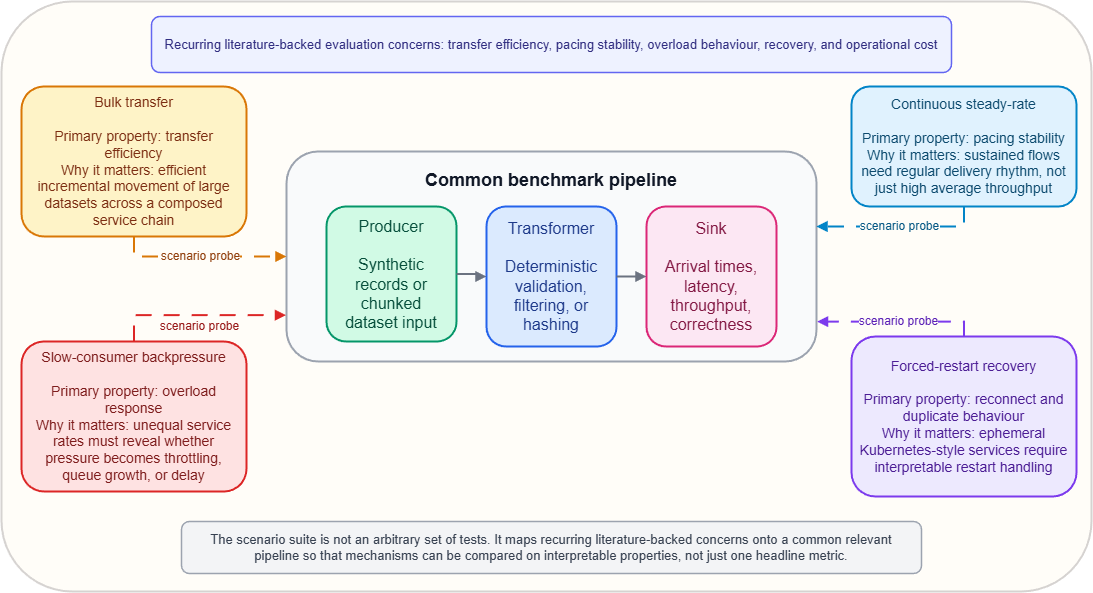
\includegraphics[width=0.92\textwidth]{figures/phase1-evaluation-map.png}
    \caption{Evaluation map showing the common benchmark pipeline and the four scenario probes used to operationalize the literature-backed evaluation dimensions.}
    \label{fig:phase1-scenario-placeholder}
\end{figure*}

\subsubsection{Experimental factors}

The independent variables cover the stress dimensions most frequently discussed in streaming-system and IPC benchmarking literature \cite{systematicstreaming,Henning2021ScalabilityMetrics,ciftci2025ipcmechanisms}: dataset size, to expose when buffering or backlog effects become significant; chunk or message size, to test the trade-off between per-message overhead and coarse-grained transfer latency; number of concurrent flows, to assess how each mechanism handles simultaneous transfers; pipeline depth, fixed here at a three-service chain so that raw transport overhead and multi-hop effects can still be distinguished; consumer speed mismatch, to expose backlog behaviour and flow-control effectiveness; resource budget, through explicit CPU and memory requests and limits for Kubernetes pods, defined as Kustomize overlay patches at three tiers (small: 100\,m\,CPU / 128\,MiB, medium: 250\,m\,CPU / 256\,MiB, large: 500\,m\,CPU / 512\,MiB); durability mode and replication factor, where the mechanism supports such trade-offs; and fault scenario, at minimum service restart during an ongoing transfer.

Not every factor needs to be crossed exhaustively. A pragmatic design is to define a core matrix over mechanism, workload profile, resource budget, and concurrency, and then use targeted follow-up experiments for failure and durability scenarios. This keeps the study manageable while still covering the trade-offs the literature treats as most important \cite{sharvari2019messaging,ciftci2025ipcmechanisms}.

\subsubsection{Result presentation and appendix boundary}

The body of the thesis should present only the compact experiment matrix and a smaller set of focused figures that are necessary for the argument. A master table can summarize each run by mechanism, workload profile, dataset size, message size, concurrency level, resource budget, and durability mode, together with the most important metrics. The main text should then highlight the most informative sweeps, such as throughput versus concurrency, latency percentiles versus message size, and recovery behaviour by failure scenario. Full preset definitions, per-run outputs, and secondary plots should be moved to an appendix so that the chapter remains analytically clear rather than turning into an undifferentiated lab log.

\subsection{gRPC Baseline Results}

\subsubsection{Metrics definitions}

Before presenting results, it is important to define the metrics used throughout the evaluation so that tables, figures, and prose refer to consistent quantities.

\begin{itemize}
    \item \textbf{Throughput (msg/s)} is the number of messages successfully received by the sink per second of wall-clock time, averaged over the entire run.
    \item \textbf{Throughput (MiB/s)} is the data volume received by the sink per second, computed as $(\mathrm{msg}/\mathrm{s}) \times \mathrm{message\ size}$.
    \item \textbf{Latency percentiles ($p_{50}$, $p_{95}$, $p_{99}$, max)} describe end-to-end message delivery delay from producer send to sink receipt. The $p_{95}$ latency, for example, means that 95\% of messages were delivered within that time or less.
    \item \textbf{Inter-arrival time} is the elapsed time between consecutive message arrivals at the sink. The $p_{95}$ inter-arrival time captures near-worst-case spacing between deliveries.
    \item \textbf{Jitter} is defined as the standard deviation of the inter-arrival times. Lower jitter indicates a more regular, predictable delivery rhythm.
    \item \textbf{Duplicates} is the number of messages received more than once by the sink. In a correct delivery, this count is zero.
    \item \textbf{Ordering violations} is the number of messages received out of their original send order.
    \item \textbf{CPU usage (\%)} is the average and peak CPU consumption per role (producer, transformer, sink), sampled at two-second intervals via \texttt{kubectl top pods} during the focused Kubernetes reruns and computed as a percentage of a single core.
    \item \textbf{Memory usage (MiB)} is the average and peak resident memory per role, sampled on the same interval.
    \item \textbf{Time to first post-failure message (ms)} is the wall-clock time between the estimated failure instant and the first message that reaches the sink afterwards.
    \item \textbf{End-to-end recovery time (ms)} is the time required for the sink to observe three consecutive one-second windows at or above 90\% of the target rate. If that threshold is never met before the run completes, the metric is capped at the backlog-drain time and reported together with a boolean indicating that the target rate was not recovered.
    \item \textbf{Backlog drain time (ms)} is the time between the estimated failure instant and the arrival of the final message for the run.
\end{itemize}

\subsubsection{Current comparison scope}

The currently completed implementation covers three transport mappings in the same three-stage pipeline (\emph{Producer} $\rightarrow$ \emph{Transformer} $\rightarrow$ \emph{Sink}): \emph{client-streaming gRPC}, \emph{unary gRPC}, and \emph{RabbitMQ Streams}. The two gRPC variants remain informative because unary approximates the current direct request-response style used in DYNAMOS, whereas client-streaming represents the most direct streaming extension of that model. RabbitMQ Streams adds a broker-mediated reference point in which the producer publishes into a durable stream and the downstream stages consume through the broker rather than over a single long-lived RPC. Kafka and NATS remain future work.

The current benchmark corpus is a completed single-repeat comparable suite executed on the same single-node Kubernetes environment for all three transports. Two clean workload families were used for the baseline matrix. The first uses synthetic payloads with message sizes from 256 bytes to 16 KiB and concurrency levels from 1 to 16. The second replays rows from copied DYNAMOS CSV datasets by batching either 25 or 100 rows into one message at concurrency 1 and 8. In addition to these clean matrices, three focused stress scenarios were executed on the same environment: a continuous steady-rate scenario, a slow-consumer backpressure scenario, and a recovery scenario with a forced mid-run transformer restart. The sink records throughput, end-to-end latency percentiles, inter-arrival behaviour, and correctness counters for every run.

This unified execution scope makes the current tables directly comparable across all three implemented transports, but it introduces a different limitation: the results are now a single-pass benchmark suite rather than repeated averages. The values reported below therefore establish a coherent comparison point for the present prototype, but they should be interpreted as point estimates rather than variance-aware performance envelopes. The CSV replay workload also still uses truncated test copies of the copied DYNAMOS CSVs because the full files exceed practical ConfigMap size limits in the current cluster setup.

\begin{table}[t]
    \centering
    \footnotesize
    \caption{Completed clean-workload summary for the single-repeat three-transport benchmark suite.}
    \label{tab:grpc-preliminary-results}
    \resizebox{\columnwidth}{!}{%
    \begin{tabular}{llll}
        \toprule
        Workload & Transport mode & Avg. throughput (msg/s) & Avg. $p_{95}$ latency (ms) \\
        \midrule
        Synthetic & Client-streaming & 49,528.87 & 107.33 \\
        Synthetic & Unary & 3,057.86 & 1.31 \\
        Synthetic & RabbitMQ Streams & 505.05 & 465.63 \\
        CSV replay & Client-streaming & 23,635.15 & 52.76 \\
        CSV replay & Unary & 2,319.08 & 0.85 \\
        CSV replay & RabbitMQ Streams & 380.53 & 388.59 \\
        \bottomrule
    \end{tabular}}
\end{table}

\begin{figure}[t]
    \centering
    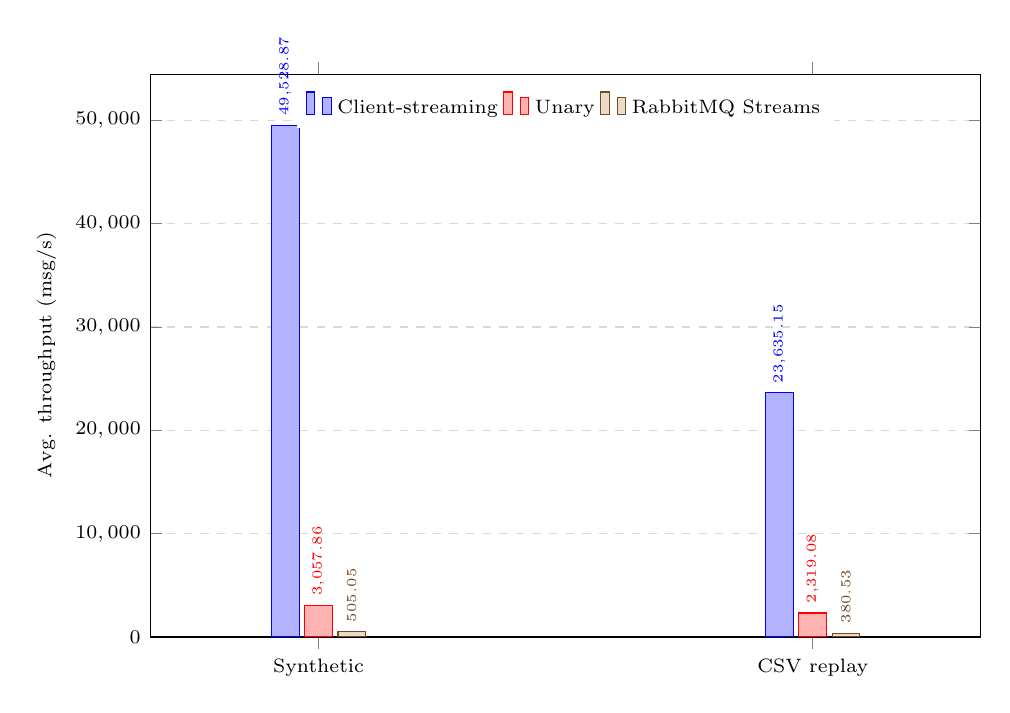
\begin{tikzpicture}
        \begin{axis}[
            ybar,
            bar width=10pt,
            width=\columnwidth,
            height=0.72\columnwidth,
            ymin=0,
            enlarge x limits=0.34,
            ylabel={Avg. throughput (msg/s)},
            symbolic x coords={Synthetic,CSV replay},
            xtick=data,
            scaled y ticks=false,
            ymajorgrids=true,
            grid style={dashed,gray!30},
            legend style={
                at={(0.5,0.98)},
                anchor=north,
                legend columns=3,
                draw=none,
                font=\scriptsize
            },
            yticklabel style={font=\scriptsize,/pgf/number format/fixed,/pgf/number format/precision=0,/pgf/number format/1000 sep={,}},
            xticklabel style={font=\scriptsize},
            ylabel style={font=\scriptsize},
            nodes near coords,
            every node near coord/.append style={font=\tiny, rotate=90, anchor=west},
            point meta=y,
        ]
            \addplot coordinates {(Synthetic,49528.87) (CSV replay,23635.15)};
            \addplot coordinates {(Synthetic,3057.86) (CSV replay,2319.08)};
            \addplot coordinates {(Synthetic,505.05) (CSV replay,380.53)};
            \legend{Client-streaming,Unary,RabbitMQ Streams}
        \end{axis}
    \end{tikzpicture}
    \caption{Average throughput for the completed clean-workload matrix, split by workload family and transport mode. Client-streaming sustains substantially higher throughput than the other currently implemented transports in both workload families.}
    \label{fig:grpc-preliminary-throughput}
\end{figure}

\subsubsection{Clean baseline matrix}

Table~\ref{tab:grpc-per-size} breaks the synthetic bulk-transfer results down by message size, averaging across concurrency levels 1, 4, 8, and 16 for each size. This disaggregation shows that the client-streaming advantage is strongly size-dependent: it delivers roughly $26.4\times$ the throughput of unary at 256~B, but that advantage narrows to about $5.6\times$ at 16~KiB as the unary path amortises part of its per-call overhead. RabbitMQ Streams occupies a different operating region entirely: its message throughput remains nearly flat at roughly 467--535 messages per second across the full size sweep, so larger payloads mainly increase MiB/s rather than message rate.

\begin{table}[t]
    \centering
    \scriptsize
    \caption{Synthetic bulk-transfer throughput by message size, averaged across concurrency levels 1, 4, 8, and 16 in the completed single-repeat suite.}
    \label{tab:grpc-per-size}
    \setlength{\tabcolsep}{3pt}
    \resizebox{\columnwidth}{!}{%
    \begin{tabular}{lrrrrrr}
        \toprule
        Msg size & \shortstack{Stream\\msg/s} & \shortstack{Unary\\msg/s} & \shortstack{RabbitMQ\\msg/s} & \shortstack{Stream\\MiB/s} & \shortstack{Unary\\MiB/s} & \shortstack{RabbitMQ\\MiB/s} \\
        \midrule
        256 B   & 97{,}182 & 3{,}682 & 535 & 23.73 & 0.90 & 0.13 \\
        1 KiB   & 60{,}676 & 3{,}418 & 522 & 59.25 & 3.34 & 0.51 \\
        4 KiB   & 27{,}462 & 2{,}856 & 467 & 107.27 & 11.16 & 1.82 \\
        16 KiB  & 12{,}795 & 2{,}276 & 496 & 199.93 & 35.56 & 7.76 \\
        \bottomrule
    \end{tabular}}
\end{table}

Three observations stand out. First, client-streaming throughput in msg/s drops substantially with payload size (from 97{,}182 to 12{,}795), but its data rate still rises from 23.73 to 199.93~MiB/s because larger messages amortise per-message overhead more effectively. Unary msg/s is much flatter across sizes (2{,}276--3{,}682), indicating that per-call overhead remains its main bottleneck. RabbitMQ Streams stays far below both direct RPC modes in msg/s, but its MiB/s rises from 0.13 to 7.76 as the broker path benefits from larger payloads.

Second, the clean workload averages in Table~\ref{tab:grpc-preliminary-results} show a consistent ordering across both workload families: client-streaming is the throughput leader, unary is the lower-latency direct RPC mode, and RabbitMQ Streams is markedly slower while also carrying a much higher average $p_{95}$ latency. In the CSV replay workload, client-streaming still outperforms unary by roughly $10.2\times$ in throughput and RabbitMQ Streams by roughly $62\times$, suggesting that the overall ranking does not depend on purely synthetic payloads.

Third, all completed clean-matrix runs preserved correctness. No duplicate deliveries or ordering violations were observed for any transport in the synthetic-clean or CSV-replay-check presets. The current baseline trade-off is therefore not correctness versus performance, but which transport pays for throughput with latency, buffering, or broker cost.

The clean matrices alone, however, are not enough to judge whether a transport is suitable for long-lived, policy-constrained data exchange. DYNAMOS-style workflows also care about pacing regularity, behaviour under consumer mismatch, and failure recovery. Three focused stress scenarios were therefore added after the baseline.

\subsubsection{Focused stress scenarios}

\paragraph{Continuous steady-rate scenario.}

The first focused experiment was a continuous steady-rate scenario. It used 1 KiB synthetic messages, a fixed target rate of 1,000 messages per second, and concurrency levels of 4 and 8, without artificial sink delay or injected failures. The goal was to measure not just throughput and latency, but also inter-arrival regularity under a long-running steady stream.

\begin{table}[t]
    \centering
    \scriptsize
    \caption{Continuous steady-rate scenario from the completed single-repeat three-transport suite.}
    \label{tab:grpc-continuous-results}
    \setlength{\tabcolsep}{3pt}
    \resizebox{\columnwidth}{!}{%
    \begin{tabular}{lrrrrr}
        \toprule
        Transport mode & Concur. & Throughput & Avg. $p_{95}$ & \shortstack{$p_{95}$ inter-\\arrival} & Jitter \\
        \midrule
        Client-streaming & 4 & 1,016.80 & 8.82 & 1.59 & 0.66 \\
        Client-streaming & 8 & 995.35 & 6.85 & 1.55 & 0.67 \\
        Unary & 4 & 1,049.43 & 1.66 & 2.12 & 2.06 \\
        Unary & 8 & 918.58 & 2.71 & 2.15 & 1.55 \\
        RabbitMQ Streams & 4 & 504.41 & 769.51 & 3.21 & 6.88 \\
        RabbitMQ Streams & 8 & 471.69 & 627.62 & 4.90 & 7.85 \\
        \bottomrule
    \end{tabular}}
\end{table}

    In this single-repeat continuous scenario, both gRPC modes stay near the 1,000 msg/s target, but they shape the flow differently. Client-streaming maintains the tighter delivery rhythm in both concurrency settings: its jitter remains near 0.66--0.67 ms and its $p_{95}$ inter-arrival delay stays near 1.55--1.59 ms. Unary keeps the lower end-to-end latency, with $p_{95}$ values between 1.66 and 2.71 ms instead of 6.85--8.82 ms for client-streaming, but its pacing is less regular. RabbitMQ Streams falls into a different regime altogether. Throughput drops to 472--504 msg/s and $p_{95}$ latency rises to 628--770 ms, while inter-arrival jitter grows sharply. In other words, the brokered path does preserve a steady sink feed, but it no longer does so at a rate or latency level that matches the direct RPC paths.

\paragraph{Slow-consumer backpressure scenario.}

The second focused experiment was a backpressure scenario. It used the same 1 KiB payload size with concurrency 8, but the single sink instance was slowed down by adding a 2\,ms processing delay per message while the producer still targeted 4{,}000 messages per second. Because the sink can process at most $\lfloor 1000/2 \rfloor = 500$ messages per second per connection, the aggregate theoretical sink capacity is $500 \times 8 = 4{,}000$ messages per second, which means the scenario operates at the boundary of the sink's processing budget. Any transport overhead or scheduling jitter pushes the effective throughput below the requested rate, causing messages to accumulate either in the gRPC transport buffers of the transformer or in the RabbitMQ broker path. This scenario was designed to expose whether the transport absorbs overload through explicit throttling or through queue growth and accumulated delay.

\begin{table}[t]
    \centering
    \scriptsize
    \caption{Backpressure scenario with an intentionally slow sink in the completed single-repeat suite.}
    \label{tab:grpc-backpressure-results}
    \setlength{\tabcolsep}{3pt}
    \resizebox{\columnwidth}{!}{%
    \begin{tabular}{lrrrrr}
        \toprule
        Transport mode & Throughput & Median lat. & Avg. $p_{95}$ & \shortstack{$p_{95}$ inter-\\arrival} & Jitter \\
        \midrule
        Client-streaming & 3,459.04 & 1,311.43 & 2,044.41 & 2.13 & 0.64 \\
        Unary & 2,363.38 & 0.45 & 0.83 & 3.16 & 1.10 \\
        RabbitMQ Streams & 478.94 & 198.11 & 413.74 & 3.06 & 8.81 \\
        \bottomrule
    \end{tabular}}
\end{table}

    This scenario shows that higher throughput is not automatically the better outcome. Under backpressure, client-streaming kept the highest realized throughput at 3,459 msg/s, but it did so by allowing the pipeline to accumulate a large queue: median end-to-end latency rose to about 1.31 seconds and $p_{95}$ latency to about 2.04 seconds. Unary behaved almost oppositely. It gave up throughput, but kept latency near the sub-millisecond range for successfully delivered requests. RabbitMQ Streams throttled even harder than unary, sustaining only 479 msg/s. That stronger throttling kept its median and $p_{95}$ latencies below the client-streaming row in this particular run, but the transport also exhibited a 21.2-second maximum latency and far higher jitter. The current interpretation is therefore that client-streaming preserves bulk movement by buffering aggressively, unary protects responsiveness by throttling, and RabbitMQ Streams pays for brokered decoupling with a severe throughput collapse and a heavier long-tail backlog.

\paragraph{Forced-restart recovery scenario.}

The third focused experiment was a recovery scenario. This run used 4 KiB messages, concurrency 8, a continuous target rate of 2,000 messages per second, and a forced \textit{Transformer} restart after 3 seconds. The producer was allowed to retry up to 120 times with a 250 ms backoff. The purpose of this scenario was not to replace the main matrix, but to observe how the currently implemented transport mappings behave when the pipeline is interrupted during an active stream.

\begin{table}[t]
    \centering
    \scriptsize
    \caption{Recovery scenario with a forced transformer restart in the completed single-repeat suite.}
    \label{tab:grpc-recovery-results}
    \setlength{\tabcolsep}{3pt}
    \resizebox{\columnwidth}{!}{%
    \begin{tabular}{lrrrrrrr}
        \toprule
        Transport mode & Throughput & $p_{95}$ lat. & Duplicates & First post-fail. & E2E recovery & Backlog drain & Reached target \\
        \midrule
        Client-streaming & 1,467.13 & 28.38 & 9,145 & 0.00 & 6,000.00 & 10,632.03 & Yes \\
        Unary & 597.21 & 1.66 & 0 & 23,819.02 & 24,000.00 & 30,489.03 & Yes \\
        RabbitMQ Streams & 1,539.17 & 5,111.95 & 4,056 & 1,009.89 & 6,000.00 & 9,993.99 & Yes \\
        \bottomrule
    \end{tabular}}
\end{table}

    The recovery scenario now needs to be read from the sink rather than from the producer alone. Client-streaming resumed almost immediately after the forced restart: the first post-failure message arrived after roughly 0.003~ms, and the sink observed sustained recovery back to the target rate after 6~s. That continuity is not free, however. The current reconnect strategy replays each worker's sequence range, which produced 9,145 duplicate messages and a backlog-drain time of 10.6~s in this run. Unary shows the opposite behaviour. It remained duplicate-free and kept overall $p_{95}$ latency low for delivered requests, but it did so while the pipeline stalled for much longer: the sink saw a 23.8~s delivery gap, 24.0~s to regain the target rate, and 30.5~s to fully drain the backlog.

    RabbitMQ Streams changes the semantics rather than mirroring either gRPC row directly. Because the producer publishes into a broker, the forced \textit{Transformer} restart is not observed as a producer-side reconnect event, so the producer-side recovery counters remain near zero and are useful only as diagnostics. The sink-side outcome is still not free. In the full rerun, RabbitMQ resumed much earlier than unary, with the first post-failure message arriving after 1.01~s, and it matched client-streaming on the 6~s sustained-recovery threshold while achieving the highest overall throughput in this single run. That better bulk continuity still comes with cost: the brokered path recorded a $p_{95}$ latency of 5.11~s, a backlog-drain time of 9.99~s, and 4,056 duplicate messages. The broker therefore masks the failure from the producer and can restore bulk delivery quickly, but it still imposes a substantial end-to-end latency and duplicate cost compared with the direct gRPC options.

\subsubsection{Discussion}

The current results support a more precise conclusion than a simple "streaming beats unary" claim. In the clean bulk-transfer baseline, client-streaming is the strongest choice for high-volume inter-service data movement, with the throughput advantage over unary varying from roughly $5.6\times$ for 16~KiB messages to $26.4\times$ for 256~B messages. Unary remains the lower-latency direct RPC option, with sub-2\,ms average $p_{95}$ latency in the clean workload summaries. In the continuous scenario, client-streaming also provides the steadier delivery rhythm, whereas unary provides lower end-to-end latency with less regular pacing. In the backpressure scenario, client-streaming preserves throughput by absorbing overload as queueing delay, while unary sacrifices throughput to protect latency. Under restart stress, the prototype does not have a single dominant winner: client-streaming minimizes the visible interruption and keeps recovery latency comparatively low, RabbitMQ restores bulk throughput just as quickly and drains the backlog slightly faster, and unary remains the cleanest duplicate-free option but recovers far too slowly to be the stronger resilience mechanism overall.

RabbitMQ Streams adds a third point in this trade-off space. It preserved correctness in the clean and CSV-replay baselines and reduced producer-visible recovery events to zero under the forced transformer restart, but the sink-side results show that this does not mean recovery is free. In the clean, continuous, and backpressure scenarios it trailed the direct gRPC modes on throughput and latency, while in the forced-restart rerun it recovered bulk delivery faster than unary and roughly on par with client-streaming, albeit with materially higher latency and duplicate cost than the direct RPC paths. The broker therefore behaves less like a performance-oriented replacement for direct RPC streaming and more like a decoupling layer that changes where backlog and recovery cost are paid.

These findings already make a useful thesis contribution because they identify concrete transport trade-offs in bulk transfer, pacing regularity, overload response, and failure recovery across both direct RPC and broker-mediated transport styles. That evidence narrows the evaluation space for the remaining broker candidates and clarifies which properties later integrations into DYNAMOS must improve or preserve.

Kafka and NATS still need to be benchmarked under the same workload definitions, but the current three-transport comparison has already narrowed the design space substantially. The remainder of the thesis can therefore focus on whether other broker-based mechanisms offer meaningful gains in replay, decoupling, or backlog tolerance without further undermining the latency, recovery, and operational properties exposed here.

\subsection{Threats to Validity}

Several threats to validity should be acknowledged when interpreting the current results.

\paragraph{Internal validity.}
The current benchmark corpus is a single-repeat suite, so no confidence intervals or variance estimates are reported for the main tables. The results may therefore be affected by transient system-level effects such as CPU scheduling variance, garbage collection pauses, or short-lived background contention in the cluster. Short run durations also mean that the study may not capture warm-up effects or long-term stability behaviour that would emerge in sustained production workloads. The CSV replay workload still uses truncated test snapshots of the copied DYNAMOS datasets because the full files exceed practical ConfigMap size limits; the replay source cycles over the loaded rows, so the workload remains useful as a realism check, but the payload mix is narrower than in the original source data.

\paragraph{External validity.}
The benchmark uses a synthetic three-stage pipeline with lightweight deterministic logic, which does not replicate the full complexity of a DYNAMOS deployment. Real DYNAMOS chains may involve additional processing stages, policy-enforcement sidecars, and heterogeneous service implementations. Furthermore, the tests are conducted in a single-node Kubernetes cluster, whereas production DYNAMOS deployments span multiple nodes with network partitioning and scheduling constraints that may affect latency and throughput characteristics differently. The Go-based benchmark services share the same runtime and gRPC library version, so results may not generalize to polyglot microservice chains.

\paragraph{Construct validity.}
Jitter is operationalized as the standard deviation of inter-arrival times, which captures variability in delivery rhythm but does not distinguish between periodic jitter and isolated outliers. Alternative metrics such as mean absolute deviation or percentile-based spread could complement the current definition. Recovery is now operationalized with sink-side time-to-first-message, end-to-end recovery to a sustained throughput threshold, backlog-drain time, and duplicate-related counters, which captures recovery quality more faithfully than a single gap metric. That said, the definition still depends on the chosen 90\% threshold, the three-window smoothing rule, and the estimated failure timestamp derived from the configured restart point rather than a transport-native fault signal.

\section{Planned: Cross-Technology Benchmark Comparison}

The benchmark design and the completed three-transport comparison presented in section~III address the first part of \emph{RQ1}. The planned next step extends that comparison by evaluating Apache Kafka and NATS JetStream under the same workload definitions, fairness constraints, and evaluation dimensions, then revisits the current RabbitMQ findings against that broader broker set. These results will allow a structured recommendation of which mechanism best fits which workload condition, completing the answer to RQ1.

\section{Planned: Architectural Integration Design}

This section will address \emph{RQ2}: how streaming communication can be integrated into DYNAMOS' microservice architecture while preserving dynamic service composition, policy-driven orchestration, and isolation guarantees. The work will examine how the selected streaming model aligns with the data-sharing archetypes implemented by DYNAMOS, specify how streaming channels are created and torn down within dynamically composed execution chains, define how sidecar responsibilities are divided for streaming versus non-streaming traffic, and address how long-lived connections interact with policy enforcement boundaries. The output will be a documented integration design accompanied by a prototype implementation that demonstrates feasibility.

\section{Planned: System-Level Evaluation}

This section will address \emph{RQ3}: what impact streaming communication has on scalability, performance, and robustness compared to the current request-response approach under realistic workloads in DYNAMOS. The benchmark logic and evaluation dimensions established in the current study will be reused, but applied within the full DYNAMOS context rather than in an isolated benchmark pipeline. The evaluation will assess whether the trade-offs identified in the current three-transport benchmark and the later cross-technology comparison carry over to the integrated system, or whether integration-specific effects such as policy enforcement overhead, sidecar latency, or orchestration coordination dominate.

\section{Conclusion}

This thesis establishes the first empirical basis for evaluating streaming communication in DYNAMOS. The literature review narrows the relevant design space to direct gRPC streaming and broker-based alternatives such as Kafka, RabbitMQ Streams, and NATS JetStream. The completed single-repeat benchmark suite shows that client-streaming gRPC is markedly stronger for sustained bulk transfer and pacing regularity, while unary gRPC remains preferable when low per-message latency and duplicate-free delivery dominate. RabbitMQ Streams now provides a concrete broker-based reference point: it preserves correctness in the clean matrices and suppresses producer-visible recovery events, but in the current prototype it does so with much lower throughput, much higher end-to-end latency, and a visible broker resource cost. Rather than yielding a single winner, the present results identify a concrete trade-off space around throughput, regularity, overload handling, recovery, and buffering semantics.

That evidence provides a defensible benchmark baseline for the remainder of the thesis, even though the current corpus is still a single-pass suite rather than a repeated statistical study. The planned next phases extend the broker comparison beyond RabbitMQ, examine how the most promising options align with DYNAMOS' archetypes and policy model, and translate those findings into an integration design and system-level validation.

\appendices

\section{Benchmark Preset Definitions}
\label{app:presets}

This appendix documents the complete preset definitions used in the benchmark. Each preset specifies the workload family, payload configuration, concurrency level, target rate (where applicable), failure injection parameters, and resource overlay tier. The five presets are: \emph{synthetic-clean} (bulk transfer baseline), \emph{csv-replay-check} (realism validation), \emph{synthetic-continuous} (steady-rate pacing), \emph{synthetic-backpressure} (slow-consumer overload), and \emph{synthetic-recovery} (forced-restart resilience).

\begin{table}[h]
    \centering
    \scriptsize
    \caption{Benchmark presets used in the current transport study.}
    \label{tab:appendix-presets}
    \setlength{\tabcolsep}{3pt}
    \resizebox{\columnwidth}{!}{%
    \begin{tabular}{lp{2.7cm}p{3.9cm}}
        \toprule
        Preset & Key parameters & Purpose \\
        \midrule
        \texttt{synthetic-clean} & Synthetic payloads from 256 B to 16 KiB, concurrency 1--16, no injected failure & Baseline bulk-transfer throughput, latency, and correctness matrix \\
        \texttt{csv-replay-check} & Copied DYNAMOS CSV rows batched as 25 or 100 rows per message & Realism check against non-synthetic payload structure \\
        \texttt{synthetic-continuous} & 1 KiB payloads, 1{,}000 msg/s target, concurrency 4 and 8, one completed comparable run & Steady-rate pacing and jitter comparison \\
        \texttt{synthetic-backpressure} & 1 KiB payloads, 4{,}000 msg/s target, concurrency 8, 2 ms sink delay, one completed comparable run & Slow-consumer overload and queueing behaviour \\
        \texttt{synthetic-recovery} & 4 KiB payloads, 2{,}000 msg/s target, concurrency 8, transformer restart after 3 s, 120 retries at 250 ms backoff, one completed comparable run & Restart recovery, replay, and continuity analysis \\
        \bottomrule
    \end{tabular}}
\end{table}

\section{Full Run Matrix}
\label{app:run-matrix}

This appendix summarizes the canonical run scopes used in the current thesis draft. The body of the thesis presents the most decision-relevant subsets, while the benchmark result directory stores the corresponding per-run JSON, NDJSON, and CSV exports generated by the execution scripts. The current chapter is based on the completed single-repeat comparable suite across all five presets.

\begin{table}[h]
    \centering
    \scriptsize
    \caption{Execution scope of the current benchmark corpus.}
    \label{tab:appendix-run-scope}
    \setlength{\tabcolsep}{3pt}
    \resizebox{\columnwidth}{!}{%
    \begin{tabular}{lp{2.3cm}p{2.6cm}p{1.3cm}p{2.6cm}}
        \toprule
        Scope & Transports & Variable dimensions & Repetitions & Role in thesis \\
        \midrule
        Synthetic clean matrix & Client-streaming, unary, rabbitmq-streams & Payload size and concurrency sweep & 1 & Main bulk-transfer baseline in Section III \\
        CSV replay check & Client-streaming, unary, rabbitmq-streams & Batch size and concurrency subset & 1 & Realism validation against copied DYNAMOS datasets \\
        Focused continuous & Client-streaming, unary, rabbitmq-streams & Concurrency 4 and 8 at fixed 1 KiB and 1{,}000 msg/s & 1 & Pacing and jitter evidence \\
        Focused backpressure & Client-streaming, unary, rabbitmq-streams & Fixed 1 KiB, concurrency 8, 4{,}000 msg/s, 2 ms sink delay & 1 & Overload and queueing evidence \\
        Focused recovery & Client-streaming, unary, rabbitmq-streams & Fixed 4 KiB, concurrency 8, forced transformer restart & 1 & Recovery and replay evidence \\
        \bottomrule
    \end{tabular}}
\end{table}

\section{Resource Utilisation Details}
\label{app:resource-details}

This appendix summarizes the resource metrics for the completed single-repeat Kubernetes suite where CPU and memory data are most informative. For RabbitMQ Streams, the broker is reported as a separate role because its buffering layer is a core part of the transport cost. The backpressure preset produced too few stable \texttt{kubectl top} samples to support a meaningful per-role comparison across all transports, so the appendix focuses on the continuous and recovery scenarios.

\begin{table}[h]
    \centering
    \scriptsize
    \caption{Continuous scenario CPU usage by role (avg./peak \%).}
    \label{tab:appendix-continuous-cpu}
    \setlength{\tabcolsep}{3pt}
    \resizebox{\columnwidth}{!}{%
    \begin{tabular}{lrrrrr}
        \toprule
        Mode & Concur. & Producer & Transformer & Sink & Broker \\
        \midrule
        Client-streaming & 4 & 23.40 / 23.40 & 8.99 / 24.20 & 5.61 / 14.90 & -- \\
        Client-streaming & 8 & -- & 9.31 / 25.60 & 5.64 / 15.50 & -- \\
        Unary & 4 & 35.70 / 35.70 & 17.88 / 39.10 & 11.12 / 24.10 & -- \\
        Unary & 8 & -- & 15.54 / 33.70 & 9.72 / 20.90 & -- \\
        RabbitMQ Streams & 4 & 7.92 / 8.30 & 9.87 / 15.60 & 6.91 / 10.90 & 29.88 / 43.30 \\
        RabbitMQ Streams & 8 & 7.88 / 8.20 & 10.46 / 15.80 & 7.50 / 11.70 & 33.00 / 46.50 \\
        \bottomrule
    \end{tabular}}
\end{table}

\begin{table}[h]
    \centering
    \scriptsize
    \caption{Recovery scenario CPU usage by role (avg./peak \%).}
    \label{tab:appendix-recovery-cpu}
    \setlength{\tabcolsep}{3pt}
    \resizebox{\columnwidth}{!}{%
    \begin{tabular}{lrrrr}
        \toprule
        Mode & Producer & Transformer & Sink & Broker \\
        \midrule
        Client-streaming & 31.60 / 31.60 & 12.64 / 31.60 & 3.89 / 17.50 & -- \\
        Unary & 4.60 / 6.00 & 2.45 / 9.10 & 2.56 / 6.10 & -- \\
        RabbitMQ Streams & 8.84 / 10.20 & 13.38 / 17.10 & 7.51 / 13.90 & 31.76 / 49.90 \\
        \bottomrule
    \end{tabular}}
\end{table}

\begin{table}[h]
    \centering
    \scriptsize
    \caption{Recovery scenario memory usage by role (avg./peak MiB).}
    \label{tab:appendix-recovery-memory}
    \setlength{\tabcolsep}{3pt}
    \resizebox{\columnwidth}{!}{%
    \begin{tabular}{lrrrr}
        \toprule
        Mode & Producer & Transformer & Sink & Broker \\
        \midrule
        Client-streaming & 7.00 / 7.00 & 3.40 / 7.00 & 2.33 / 7.00 & -- \\
        Unary & 7.00 / 7.00 & 3.08 / 7.00 & 4.53 / 7.00 & -- \\
        RabbitMQ Streams & 10.00 / 10.00 & 25.72 / 31.00 & 5.78 / 8.00 & 490.91 / 511.00 \\
        \bottomrule
    \end{tabular}}
\end{table}

\bibliographystyle{IEEEtran}
\bibliography{references}

\end{document}